\documentclass[varwidth=true, border=2pt]{standalone}

\usepackage{pgfplots}
\usepackage{tikz}

\begin{document}
	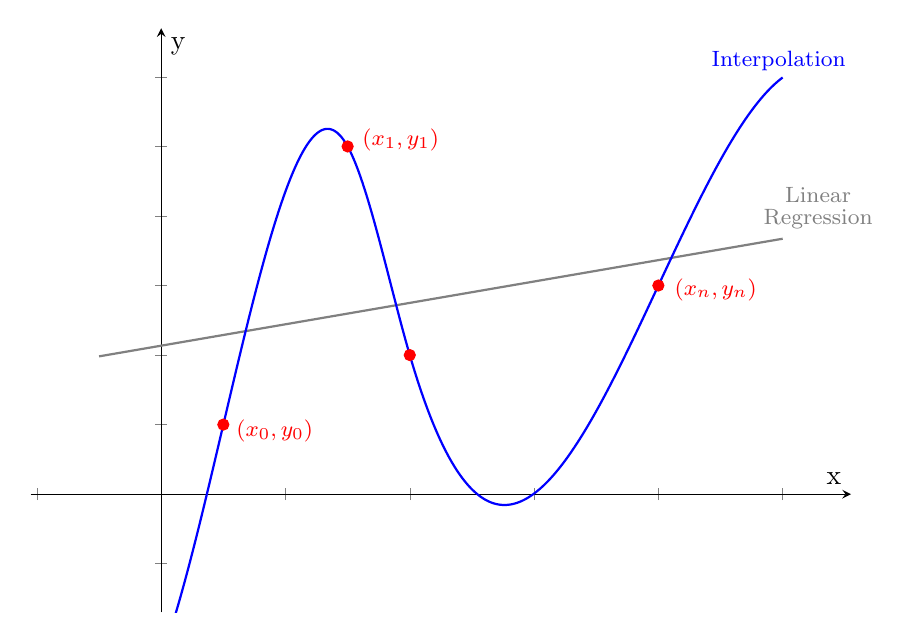
\begin{tikzpicture}
	\node[color=blue] at (9.5,7){\footnotesize{Interpolation}};
	\node[color=gray] at (10,5.3){\footnotesize{Linear}};
	\node[color=gray] at (10,5){\footnotesize{Regression}};
	\node[color=red] at (3.1,2.3) {\footnotesize{$(x_0,y_0)$}};
	\node[color=red] at (4.7,6) {\footnotesize{$(x_1,y_1)$}};
	\node[color=red] at (8.7,4.1) {\footnotesize{$(x_n,y_n)$}};

    \begin{axis}[
        legend pos=south east,
        axis x line=middle,
        axis y line=middle,
	xticklabels=\empty,
	yticklabels=\empty
        grid = none ,
        width=12cm,
        height=9cm,
        grid style={dashed, gray!1},
        xmin=-1,     % start the diagram at this x-coordinate
        xmax= 10,    % end   the diagram at this x-coordinate
        ymin=-1,     % start the diagram at this y-coordinate
        ymax= 6,   % end   the diagram at this y-coordinate
        %axis background/.style={fill=white},
        xlabel=x,
        ylabel=y,
        %xticklabels={-2,-1.6,...,2},
        %yticklabels={-8,-7,...,8},
        %tick align=outside,
        enlargelimits=true,
        tension=0.08]
        \addplot[domain=-1:10, gray, thick,samples=250] {0.1538*x+2.135}; % Linear Regression
        \addplot[domain=0:3,blue, thick,samples=250] {1+449/118*(x-1)-213/472*(x-1)*(x-1)*(x-1)}; % S0
        \addplot[domain=3:4, blue, thick,samples=125] {5-95/59*(x-3)-639/236*(x-3)*(x-3)+311/236*(x-3)*(x-3)*(x-3)}; % S1
        \addplot[domain=4:10, blue, thick,samples=250] {2-725/236*(x-4)+147/118*(x-4)*(x-4)-49/472*(x-4)*(x-4)*(x-4)}; % S2

       \addplot[red, only marks, mark=*] coordinates {(1,1)(3,5)(4,2)(8,3)};
      %\addlegendentry{$f(x)=x^3$}
    \end{axis}
\end{tikzpicture}
\end{document}